\subsection{Initial value problem}

\begin{frame}{Initial value problem}
  \begin{description}
    \item[Dane:]
      $f(x)$ ciągła dla wszystkich $x$
    \item[Szukana:]
      $u(x,t)$
      \begin{itemize}
        \item określona i ciągła \\ dla $-\infty < x < \infty, t \ge 0$
        \item spełniająca $(*)$ \\ dla $-\infty < x < \infty, t > 0$
        \item spełniająca $u(x,0) = f(x)$ \\ dla $-\infty < x < \infty, t = 0$
      \end{itemize}
  \end{description}
\end{frame}

\begin{frame}
  \centerline{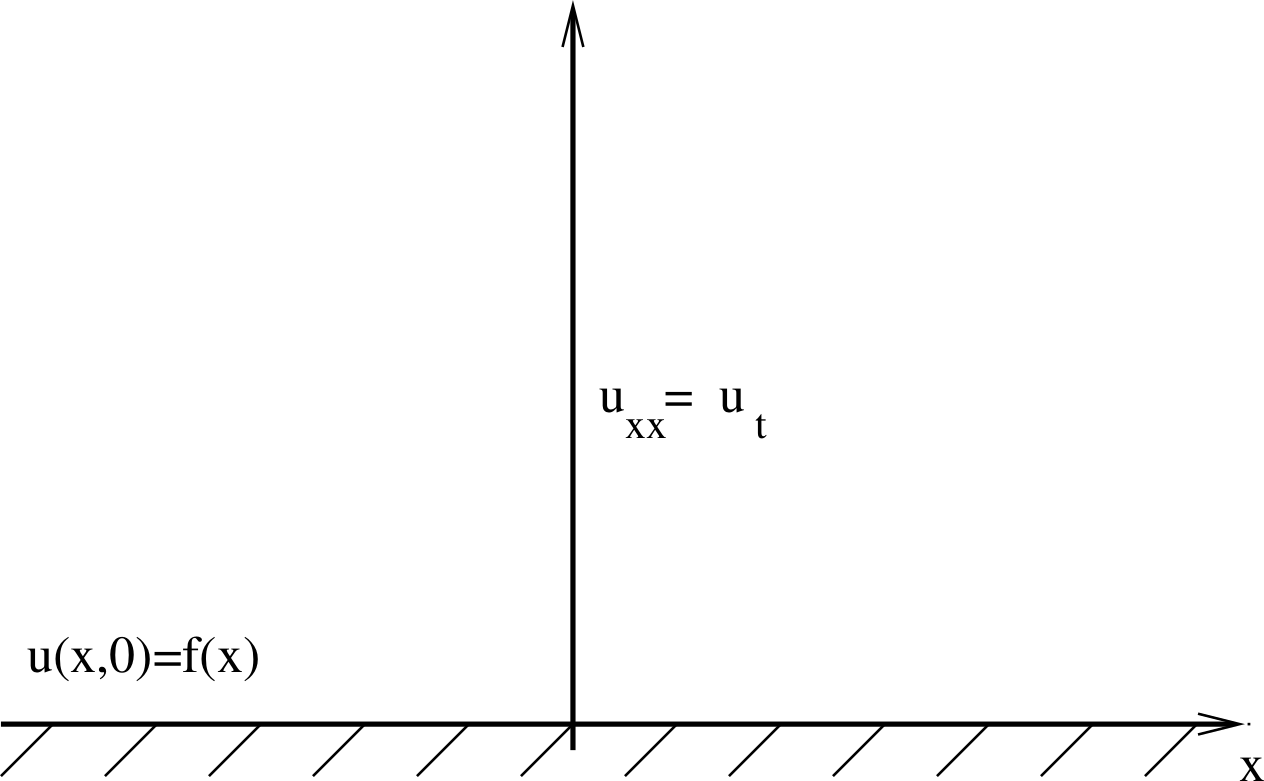
\includegraphics[height = 0.85 \textheight]{img/23/ivp}}
  (half-plane)
\end{frame}

\begin{frame}
  Rozwiązanie $\rightarrow$ całka Fouriera
  \begin{alertblock}{Problem}
    \begin{itemize}
      \item przypadek nieliniowy $\rightarrow$ ?
      \item kłopoty z wyznaczeniem wartości w $(x,t)$
    \end{itemize}
  \end{alertblock}
\end{frame}
